%%%%%%%%%%%%%%%%%%%%%%%%%%%%%%%%%%%%%%%%%%%%%%%%%%%%%%%%%%%%%%%%%%%%%%
% LaTeX Example: Project Report
%
% Source: http://www.howtotex.com
%
% Feel free to distribute this example, but please keep the referral
% to howtotex.com
% Date: March 2011
%
%%%%%%%%%%%%%%%%%%%%%%%%%%%%%%%%%%%%%%%%%%%%%%%%%%%%%%%%%%%%%%%%%%%%%%
% How to use writeLaTeX:
%
% You edit the source code here on the left, and the preview on the
% right shows you the result within a few seconds.
%
% Bookmark this page and share the URL with your co-authors. They can
% edit at the same time!
%
% You can upload figures, bibliographies, custom classes and
% styles using the files menu.
%
% If you're new to LaTeX, the wikibook is a great place to start:
% http://en.wikibooks.org/wiki/LaTeX
%
%%%%%%%%%%%%%%%%%%%%%%%%%%%%%%%%%%%%%%%%%%%%%%%%%%%%%%%%%%%%%%%%%%%%%%
% Edit the title below to update the display in My Documents
%\title{Project Report}
%
%%% Preamble
\documentclass[paper=a4, fontsize=11pt,linespread=1.5]{scrartcl}
\usepackage[T1]{fontenc}
\usepackage{fourier}
\usepackage[english]{babel}															% English language/hyphenation
\usepackage[protrusion=true,expansion=true]{microtype}	
\usepackage{amsmath,amsfonts,amsthm} % Math packages
\usepackage[pdftex]{graphicx}	
\usepackage{url}
%\usepackage{marginnote}
\usepackage{bm}
\usepackage{graphicx}
\usepackage{color}
%%% Custom sectioning
\usepackage{sectsty}
\allsectionsfont{\centering \normalfont\scshape}


%%% Custom headers/footers (fancyhdr package)
\usepackage{fancyhdr}
\pagestyle{fancyplain}
\fancyhead{}											% No page header
\fancyfoot[L]{}											% Empty
\fancyfoot[C]{}											% Empty
\fancyfoot[R]{\thepage}									% Pagenumbering
\renewcommand{\headrulewidth}{0pt}			% Remove header underlines
\renewcommand{\footrulewidth}{0pt}				% Remove footer underlines
\setlength{\headheight}{13.6pt}


%%% Equation and float numbering
\numberwithin{equation}{section}		% Equationnumbering: section.eq#
\numberwithin{figure}{section}			% Figurenumbering: section.fig#
\numberwithin{table}{section}				% Tablenumbering: section.tab#


%%% Maketitle metadata
\newcommand{\horrule}[1]{\rule{\linewidth}{#1}} 	% Horizontal rule

\title{
		%\vspace{-1in} 	
		\usefont{OT1}{bch}{b}{n}
		\normalfont \normalsize \textsc{Tsinghua University} \\ [25pt]
		\horrule{0.5pt} \\[0.4cm]
		\huge Drug Identification by Maximizing Information Flow \\
		\horrule{2pt} \\[0.5cm]
}
\author{
		\normalfont 								\normalsize
        Bingjie Zhou\\[-3pt]		\normalsize
        \today
}
\date{}

\linespread{1.5}
%%% Begin document
\begin{document}
\maketitle
\begin{abstract}
The abstract should be a brief summary of your results that grabs the reader��s attention.It is the first thing the reader will see, and you must convince the reader that the rest of your paper is worthwhile. In the best of all possible worlds, L ATEX will take care of all the formatting for you. Let v = (v0, v1, . . . , vn). If your abstract  contains nothing but words, no one would know that you��re using L ATEX!
\end{abstract}
\newpage
\tableofcontents
\newpage
%\section{Introduction}
%\section{Data}
\section{Introduction}
\begin{flushleft}
\item Drug target is the native protein in the body whose activity is modified by a drug resulting in a specific effect.[1] Over eighty percent of targets are protein and almost fifty percent are belong to GPCRs, serine, threonine and protein tyrosine kinase, MMPs, serine protease, hormone nuclear receptor and PDEs, these six families and in theory, proteins act as drug targets must be capable of combining small molecules associated to diseases with appropriate chemical characters and affinity and could express in pathology cells and tissues resulting in therapeutic effect.[2] So as long as we find a specific target, we could develop and design drugs using it��s structure and characteristics. For example, cosmopolitan conundrum Alzheimer��s disease, one of serious threats to health among modern elderly, has complex etiology and its attack related to many segments which provides lots of target spots to uncover targets . Finally people found drugs corresponded to these targets like donepezil.[2] Moreover, we could have a further research about side
effects and toxicities of drugs which are also caused by unwanted adversed effect of targets.

~\\
Commonly, we think that one drug acts selectively to one specific target.However, we are revealing a far more complex figure of drug reaction in the past decades.An elegant new theory by Yildirim illustrates that not only that there are multiple drugs relating to one target but that one target could associate to many drugs.[3] This theory provided us chance to look drug actions as networks which improves our discovery of targets by drug-drug and protein-protein associations.Although many effective analysis were evidenced past such as phenotypic effect-based approaches which is based on phenotypic responses to external compounds and chemical structure-based approaches which integrate drug chemical similarities and protein sequence or structure information, there are apparently shortcomings��for phenotypic approach, similar responses may due to similar pathway or biological process instead of same target and expression could not distinguish target from downstream genes; for chemical approach, we do not have enough prior information for major chemicals. So there is urgent necessary to combine phenotypic and chemical indexes together and achieve new method to predict drug-target association in large scale.[4]Cipher model was proposed and validated as the most accurate way to the prediction.

~\\
In Cipher model, it is assumed that similarities in pharmacological space termed as Therapeutic Similarities(TS) and drug chemical similarities(CS) are correlated with the relatedness of targets based on protein-protein interaction(PPI) network in genomic space.Based on this assumption, a computational framework drugCipher was built to relate pharmacological and genomic spaces with multi-dimentional information and used three linear regression models to calculate concordance scores which used as standard of correlation between drug and protein.[4]

\newpage

\begin{figure}
\begin{center}
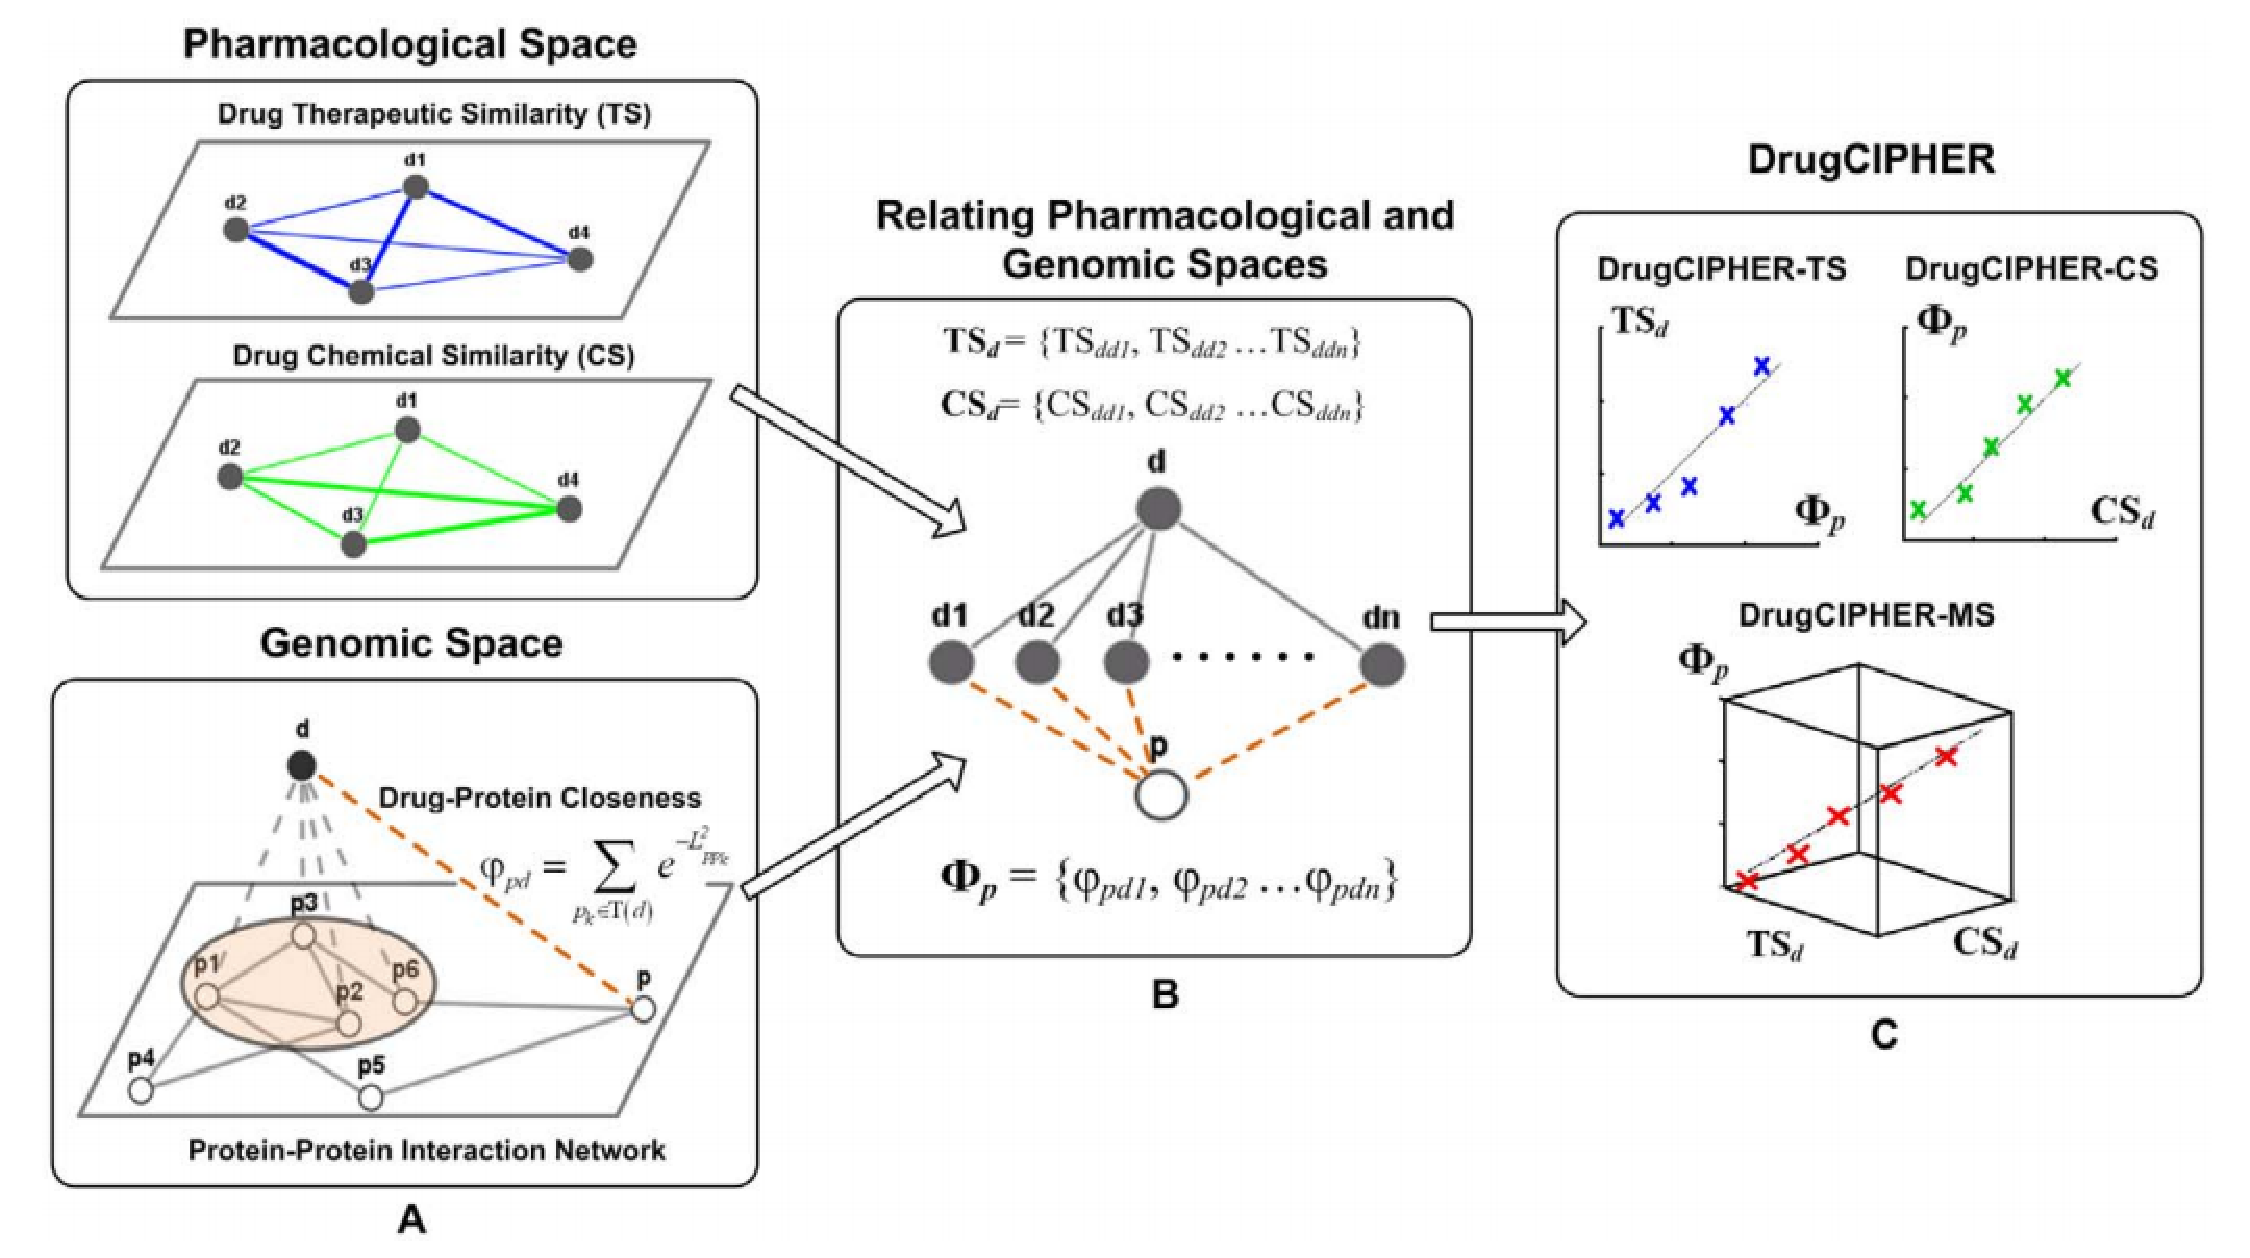
\includegraphics [width=0.8\textwidth]{drugcipher}
\end{center}
\end{figure}


\scriptsize
 \textbf{Figure 1:principle of drugCipher }Drugs are solid nodes and presented by ��d��; proteins are hollow nodes and presented by ��p��. A). Drug Therapeutic Similarity (TS) (blue solid edges) and Drug Chemical Similarity (CS) (green solid edges) comprise the pharmacological space. The protein protein interaction (PPI) (gray solid edges) network represents the information in the genomic space. Together with drug-target interactions (gray dashed edges), the closeness (brown dashed edges) is defined to associate a drug with any arbitrary protein. B). For drug d and protein p, two similarity vectors for d in pharmacological space (TSd and CSd) and one closeness vector for p (Wp) are constructed. C. The concordance scores between drug d and protein p are computed based on three linear regression models, which assume linear correlations exist between TSd and Wp,Wp and CSd, Wp and the combination of TSd and CSd.[4]\

\vspace{1cm}

\normalsize
Although Cipher has a high validated sensitivity and precision score among all approaches but the linear regression model is not clear under the situation that the protein-protein interactions and drug-drug similarities are low, showing on the left, top and right, bottom part of graph. And above approaches largely depended on PPI networks to estimate similarity. Since they consider shortest path as the optimal path between proteins and proteins and overlook others paths, the reliability of the optimal path and the final result may be adversely affected.[5]
Motivated by these observations, we proposed a new combinatorial approach to calculate score of association between a pair of drug and protein in this paper.In our approach, we first introduce a threshold to select out high similarities which have biological meanings.Then we set up a drug-protein network by integrating given drug-target interactions, PPI network information and drug-drug similarity from DrugBank database.The magnitudes of associations are recorded under the assumption that drugs with high similarities have stronger associations as the capacity of each edge for final calculation. Then we will judge the strength of the relation based on the amount of information flow between drug and protein and we will develop MAXIF(Maximizing information flow) algorithm in the drug-protein network system to figure out the path containing the maxima information and compute the max information flow as the concordance score of this pair of drug-protein. Proteins with high score are considered as potential targets.We show the accuracy and competitive of our method by series designed experiments and comparisons with other approaches and we our method to do couple of predictions as successful applications.

~\\
Once the approach is validated to be accurate, we could use it to predict potential targets which could excavate novel applications of existing drugs and narrow the range of test experiments and also work out drugs with specific curative effect.If we have enough data of targets, we could be clear of the problem of side effects so that we could avoid unwanted effects and raise efficiency of drugs.So identifying targets in a more efficient way is a stepping-stone in the discovery of pharmacology.
\end{flushleft}
\newpage
\section{Method and Materials}

Here, you will begin to present the work that you have done. What you do in this section depends on the type of work that you��re doing. For Chemistry, Biology, and other science work, for example, you may have a section labeled Materials and Methods. For math papers, the title of the section may be a particular case that you��re investigating. A good way to find ideal sections to use is to look at past RSI papers, as well as papers in your field (representative papers from recent years are in /mit/rsi/examples/papers). Additional guidance on ways to segment your paper can be found by talking to your tutor. You can also check out the RSI webpage for additional information on how to segment out
your paper.

\newpage
\section{Result}

If you need a second section of discussion, this is where you��ll put it. Perhaps you��ll need a table:

%\subsection{Simulation Test}
%\subsection{Compared with SEA}
\section{Discussion}

You can have as many major sections as is prudent. Again, look to papers in your field, past RSI papers, and RSI staff, especially your tutor, for advice. Also, think of dividing major sections into subsections as necessary. It is often more useful to have two related topics as subsections within a larger section than to have them as two
independent sections.

\section*{Reference}


\begin{thebibliography}{99}
\bibitem{[1]}Rang HP, Dale MM, Ritter JM, Flower RJ, Henderson G (2012)
\emph{"Chapter 2: How drugs act: general principles"Rang and Dale's Pharmacology.} Edinburgh; New York: Elsevier/Churchill Livingstone page 6-19 ISBN 0-7020-3471-1

\bibitem{[2]}Jianxiong Yang,Zhihui Liu,
\emph{Effect of drug targets in developing novel drugs},Lishizhe Medicine and Materia Medica Research ,vol. 20 no.3(2009)

\bibitem{[3]}Andrew L. Hopkins,
\emph{Network biology illustrates our understanding of drug actions}, Nature Biotechnology,vol 25,no.10 (October 2007)

\bibitem{[4]}Shiwen Zhao, Shao Li,
\emph{Network-based relating pharmacological and genomic spaces for drug target identification}
.Plos one ,vol 5,issue 7(July 2010)

\bibitem{[5]}Yong Chen,Tao Jiang,Shao Li,
\emph{Uncovering disease genes by maximizing information flow in the phenome-interactome network}
,Bioinformatics, vol 27, page i167-i176(2011)
\end{thebibliography}


\newpage
\section{Append}

\end{document}
